%%%%%%%%%%%%%%%%%%%%%%%%%%%%%%%%%%%%%%%%%
% Jacobs Landscape Poster
% LaTeX Template
% Version 1.0 (29/03/13)
%
% Created by:
% Computational Physics and Biophysics Group, Jacobs University
% https://teamwork.jacobs-university.de:8443/confluence/display/CoPandBiG/LaTeX+Poster
% 
% Further modified by:
% Nathaniel Johnston (nathaniel@njohnston.ca)
%
% This template has been downloaded from:
% http://www.LaTeXTemplates.com
%
% License:
% CC BY-NC-SA 3.0 (http://creativecommons.org/licenses/by-nc-sa/3.0/)
%
%%%%%%%%%%%%%%%%%%%%%%%%%%%%%%%%%%%%%%%%%

%----------------------------------------------------------------------------------------
%	PACKAGES AND OTHER DOCUMENT CONFIGURATIONS
%----------------------------------------------------------------------------------------

\documentclass[final]{beamer}

\usepackage[scale=1.24]{beamerposter} % Use the beamerposter package for laying out the poster
\usepackage[utf8]{inputenc}

\usetheme{confposter} % Use the confposter theme supplied with this template

\setbeamercolor{block title}{fg=ngreen,bg=white} % Colors of the block titles
\setbeamercolor{block body}{fg=black,bg=white} % Colors of the body of blocks
\setbeamercolor{block alerted title}{fg=white,bg=dblue!70} % Colors of the highlighted block titles
\setbeamercolor{block alerted body}{fg=black,bg=dblue!10} % Colors of the body of highlighted blocks
% Many more colors are available for use in beamerthemeconfposter.sty

%-----------------------------------------------------------
% Define the column widths and overall poster size
% To set effective sepwid, onecolwid and twocolwid values, first choose how many columns you want and how much separation you want between columns
% In this template, the separation width chosen is 0.024 of the paper width and a 4-column layout
% onecolwid should therefore be (1-(# of columns+1)*sepwid)/# of columns e.g. (1-(4+1)*0.024)/4 = 0.22
% Set twocolwid to be (2*onecolwid)+sepwid = 0.464
% Set threecolwid to be (3*onecolwid)+2*sepwid = 0.708

\newlength{\sepwid}
\newlength{\onecolwid}
\newlength{\twocolwid}
\newlength{\threecolwid}
\setlength{\paperwidth}{48in} % A0 width: 46.8in
\setlength{\paperheight}{36in} % A0 height: 33.1in
\setlength{\sepwid}{0.024\paperwidth} % Separation width (white space) between columns
\setlength{\onecolwid}{0.22\paperwidth} % Width of one column
\setlength{\twocolwid}{0.464\paperwidth} % Width of two columns
\setlength{\threecolwid}{0.708\paperwidth} % Width of three columns
\setlength{\topmargin}{-0.5in} % Reduce the top margin size
%-----------------------------------------------------------
\renewcommand{\figurename}{Fig.}

\definecolor{dorado}{RGB}{255,204,102}

\usepackage{graphicx}  % Required for including images

\usepackage{booktabs} % Top and bottom rules for tables

%----------------------------------------------------------------------------------------
%	TITLE SECTION 
%----------------------------------------------------------------------------------------

\title{CNN pre-training using convolutional autoencoders} % Poster title

\author{Russell Hoffman, Sabbir Ahmmed, Maximilian Kohlbrenner } % Author(s)

\institute{TU Berlin} % Institution(s)

%----------------------------------------------------------------------------------------

\begin{document}

\addtobeamertemplate{block end}{}{\vspace*{2ex}} % White space under blocks
\addtobeamertemplate{block alerted end}{}{\vspace*{2ex}} % White space under highlighted (alert) blocks

\setlength{\belowcaptionskip}{2ex} % White space under figures
\setlength\belowdisplayshortskip{2ex} % White space under equations

\begin{frame}[t] % The whole poster is enclosed in one beamer frame

\begin{columns}[t] % The whole poster consists of three major columns, the second of which is split into two columns twice - the [t] option aligns each column's content to the top

\begin{column}{\sepwid}\end{column} % Empty spacer column

\begin{column}{\onecolwid} % The first column

%----------------------------------------------------------------------------------------
%	OBJECTIVES
%----------------------------------------------------------------------------------------

\begin{block}{Convolutional Autoencoders}

\begin{itemize}
	\item as compared to non-conv autoenc
	\item regularization
\end{itemize}

\end{block}


\begin{block}{Experimental setup}

\begin{figure}
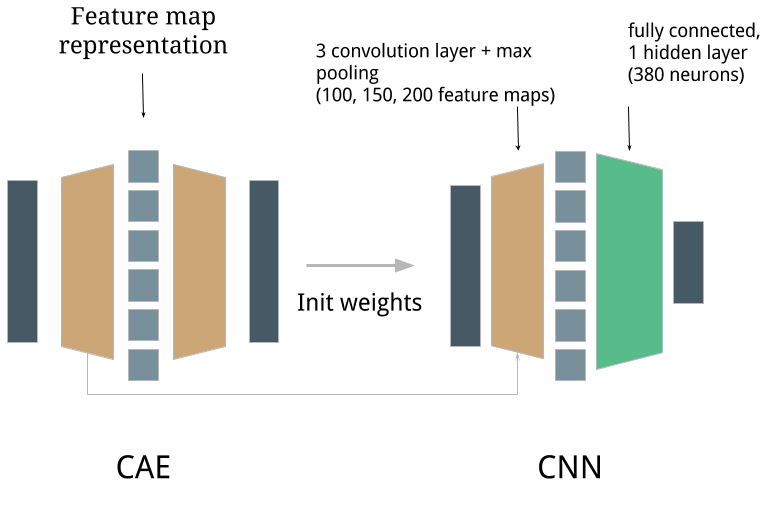
\includegraphics[width=0.8\linewidth]{graphics/setup.png}
\caption{Bisectrices de un ángulo}
\end{figure}

\end{block}

%----------------------------------------------------------------------------------------
%	INTRODUCTION
%----------------------------------------------------------------------------------------

\begin{block}{CIFAR-10}
\begin{figure}
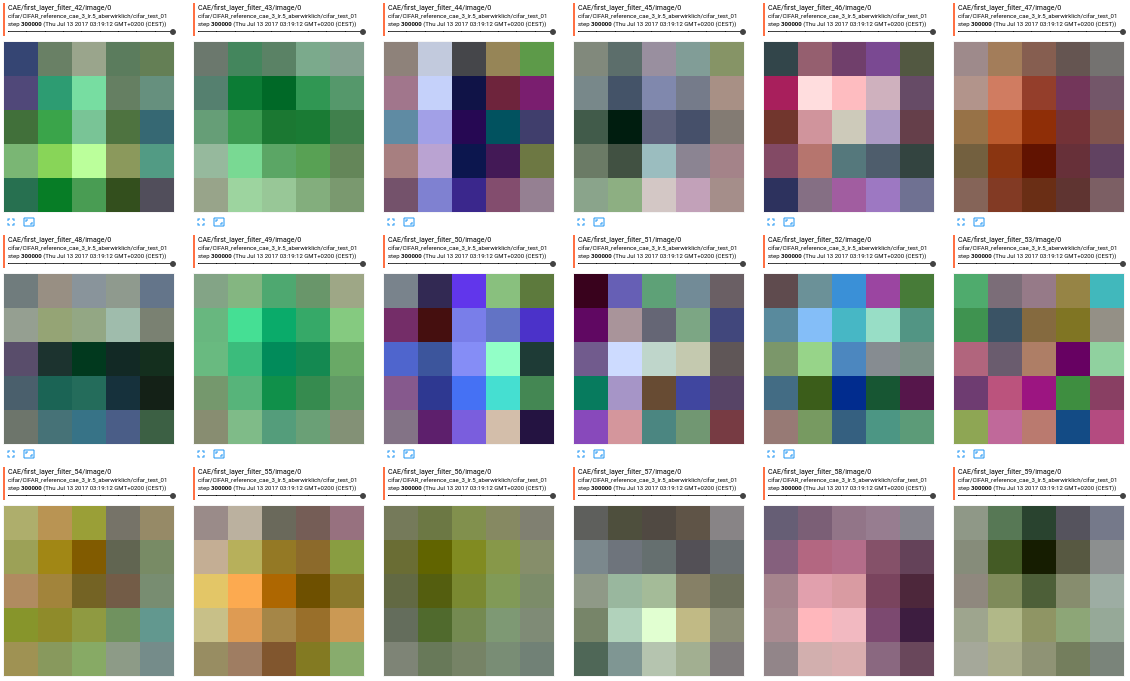
\includegraphics[width=0.8\linewidth]{graphics/cifar_filters.png}
\caption{selection of CAE first layer filters on CIFAR10}
\end{figure}

\end{block}

\setbeamercolor{block alerted title}{fg=black,bg=dorado} % Change the alert block title colors
\setbeamercolor{block alerted body}{fg=black,bg=white} % Change the alert block body colors

\begin{alertblock}{miscellaneous findings}
\begin{itemize}
	\item (pixel-wise) average cross-entropy not suited for convolutional autoencoder (useful for non-conv)
	\item max-pooling for regularization 
\end{itemize}
\end{alertblock}


\end{column} % End of the first column

% ----------------------------------------------
% SECOND COLUMN
% ----------------------------------------------


\begin{column}{\sepwid}\end{column} % Empty spacer column

\begin{column}{\onecolwid} % Begin a column which is two columns wide (column 2)

%\begin{columns}[t,totalwidth=\twocolwid] % Split up the two columns wide column

%\begin{column}{\onecolwid}\vspace{-.6in} % The first column within column 2 (column 2.1)

\begin{block}{MNIST}

\begin{figure}
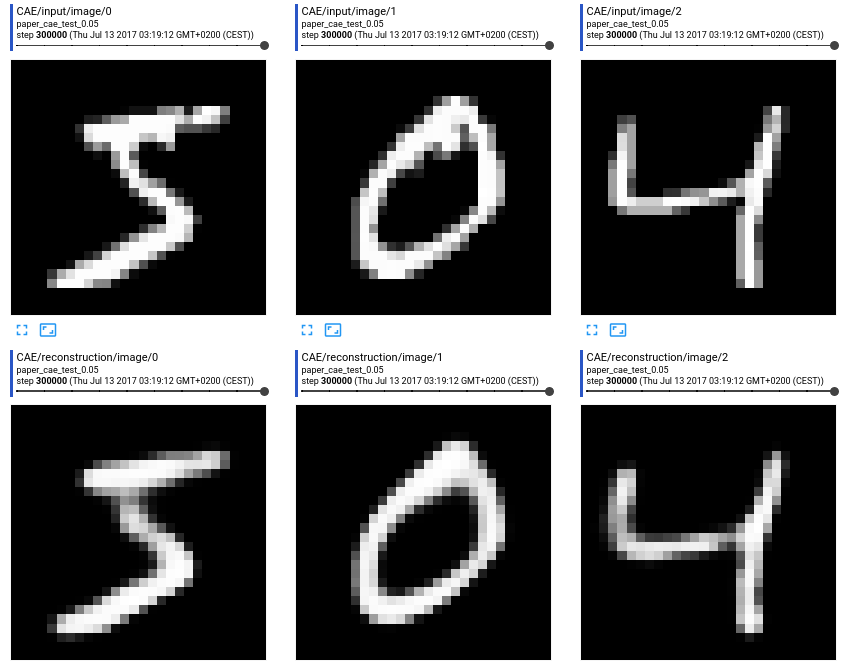
\includegraphics[width=0.8\linewidth]{graphics/mnist_reconstructions.png}
\caption{MNIST CAE reconstruction}
\end{figure}

\end{block}
%------------------------------------------------

\begin{block}{Stats}
\begin{itemize}
\item (lmage content) handwritten digits 
\item (label type) digits (0-9)
\item (datase sizes) 60k train 10k test
\item (size and colors) 28 * 28 , 1 channel (grayscale)
\item (compared difficulty) very simple (linear > 90 \% acc)
\item (SOTA performance) include Sabbir

\end{itemize}
\end{block}

\begin{block}{Experimental results}

\begin{figure}
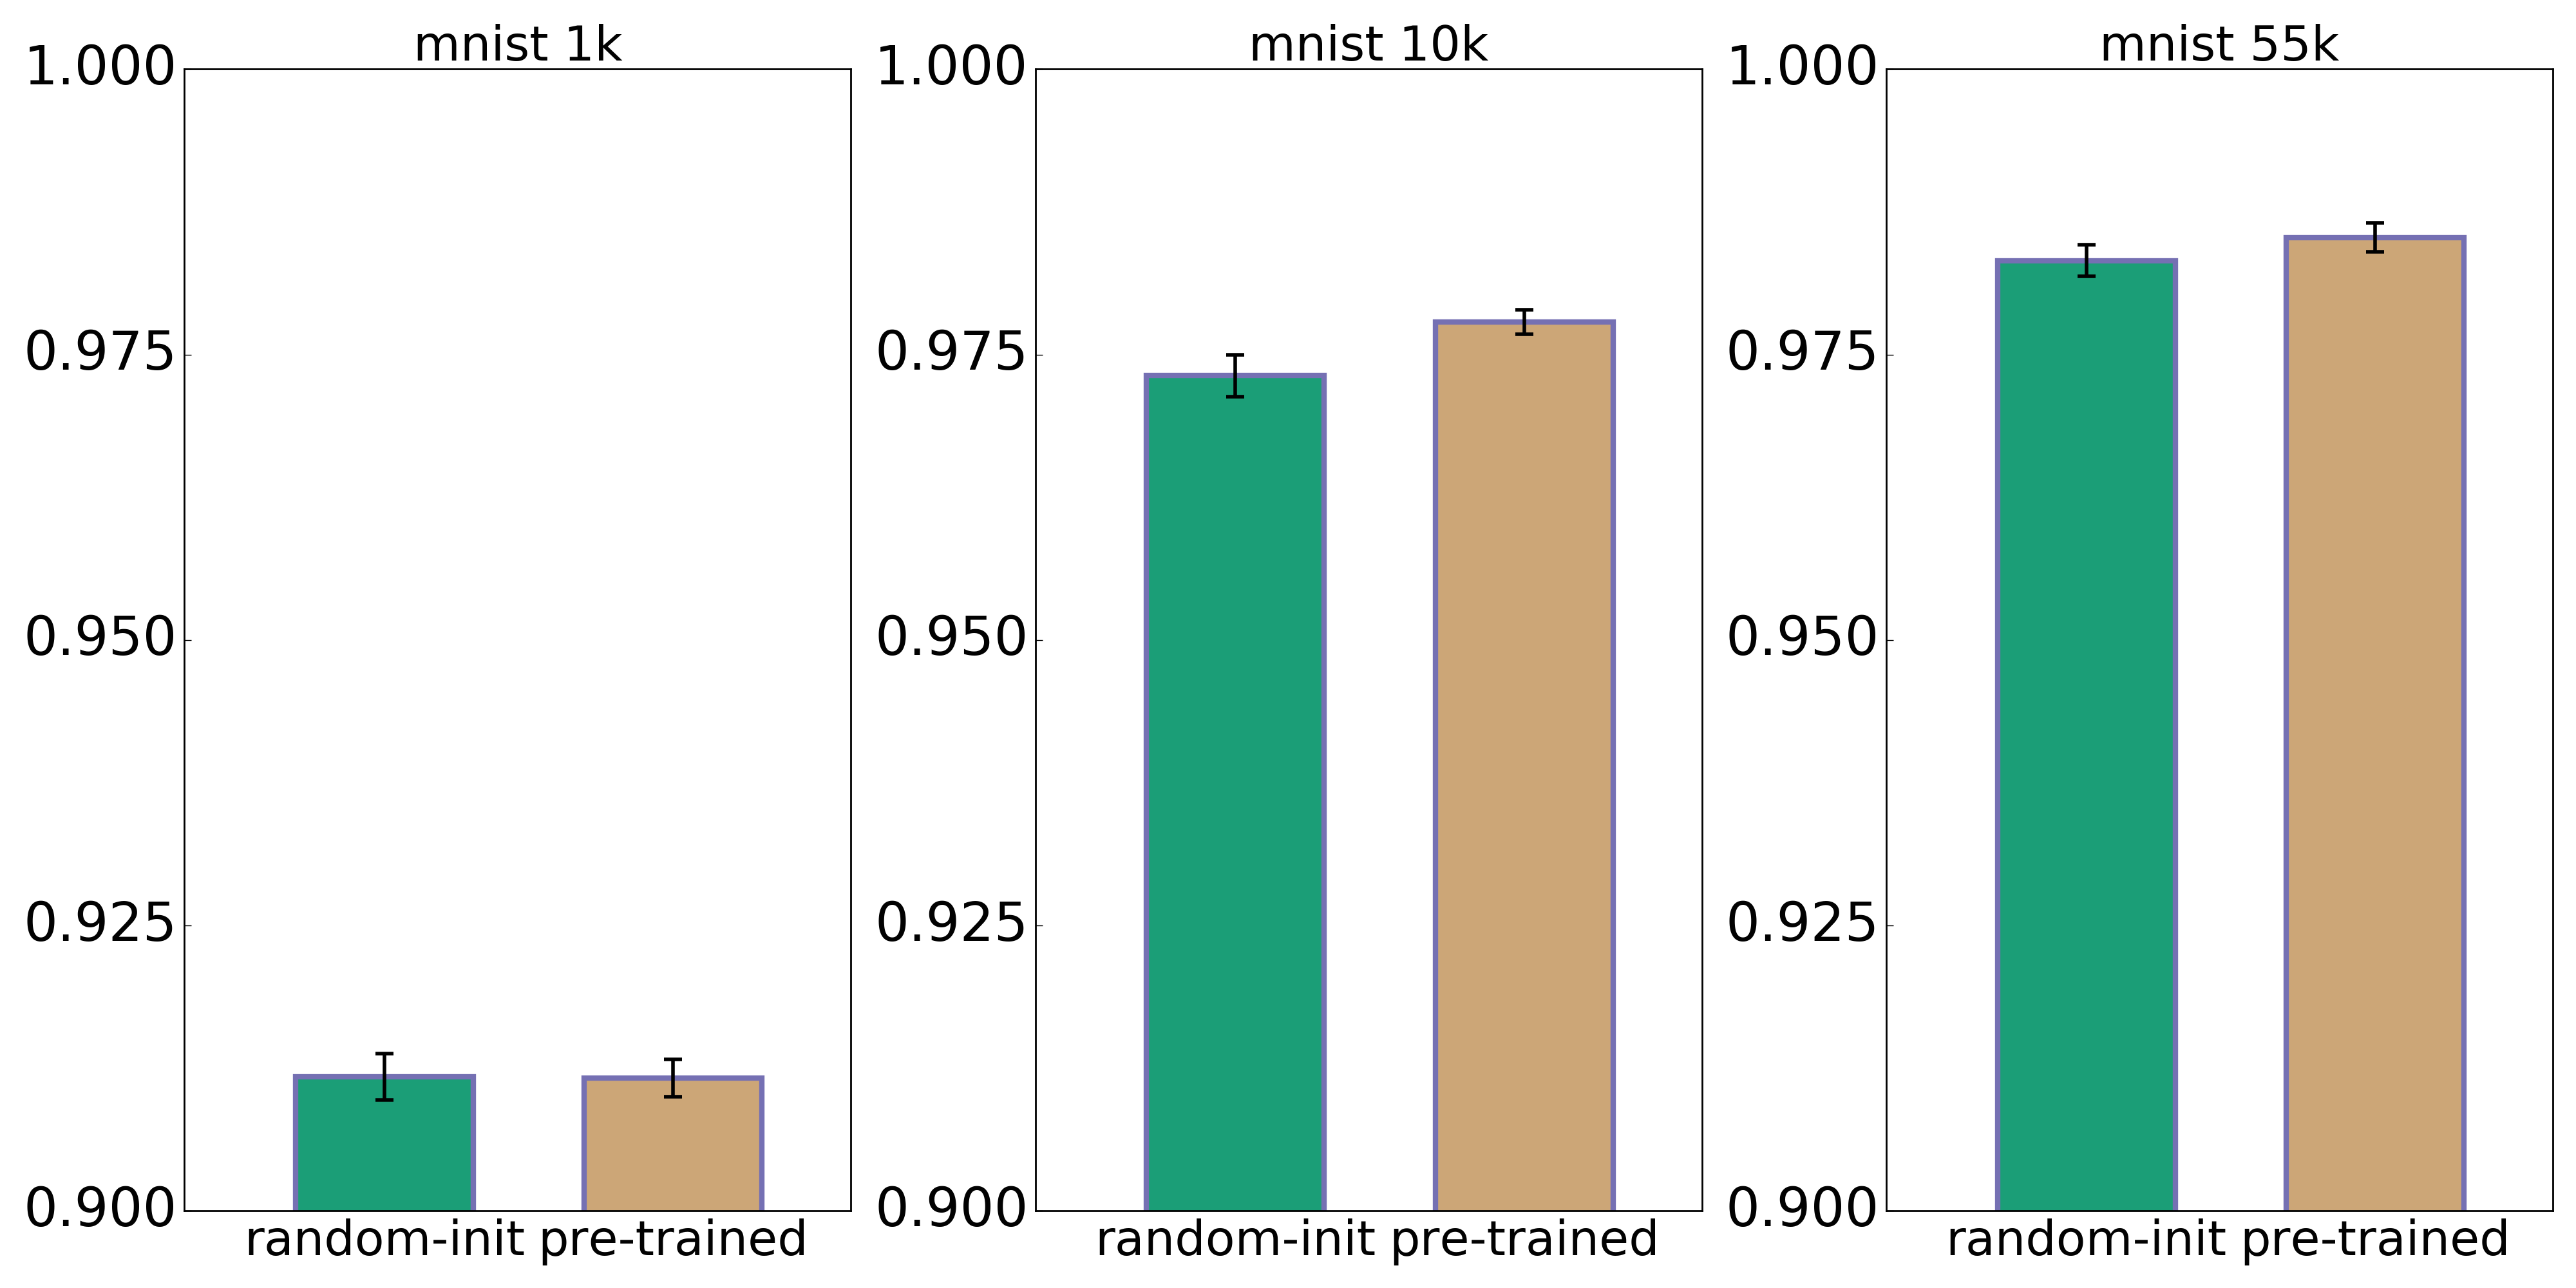
\includegraphics[width=\linewidth]{box_plots/boxplots_mnist.png}
\caption{boxplot of training accuracies}
\end{figure}

\end{block}


\end{column} % End of column 2



\begin{column}{\onecolwid} 

\begin{block}{CIFAR}

\end{block}

\begin{figure}
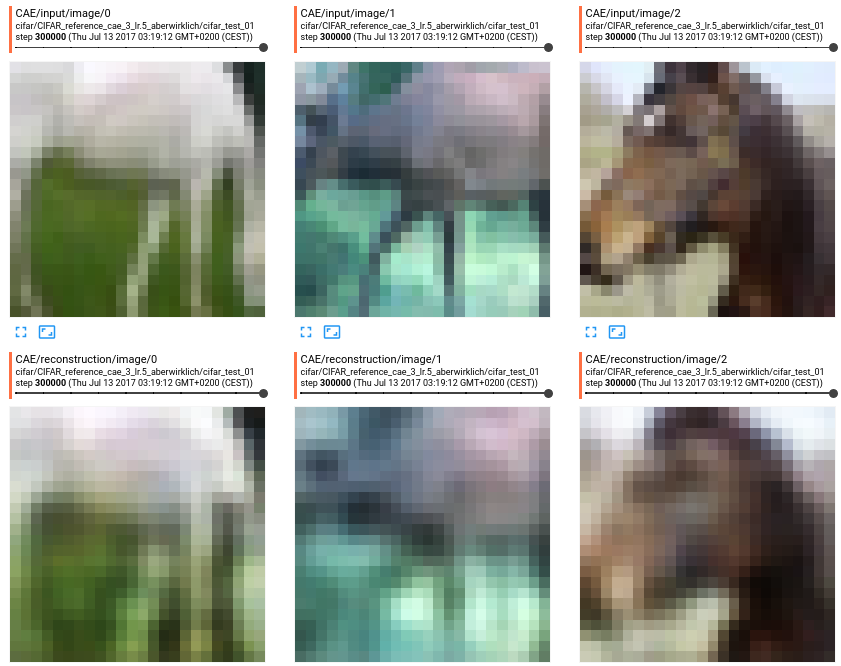
\includegraphics[width=0.8\linewidth]{graphics/cifar_reconstructions.png}
\caption{Diagrama del problema}
\end{figure}

\begin{block}{Stats}
\begin{itemize}
\item (lmage content) real-world images
\item (label type) 10 mutually exclusive categories (car, horse, cat ...)
\item (datase sizes) 50k train 10k test
\item (size and colors) 32 * 32 , 3 channel (rgb)
\item (compared difficulty) much more difficult than MNIST, color images
\item (SOTA performance) include Sabbir
\end{itemize}
\end{block}


\begin{block}{Experimental results}

\begin{figure}
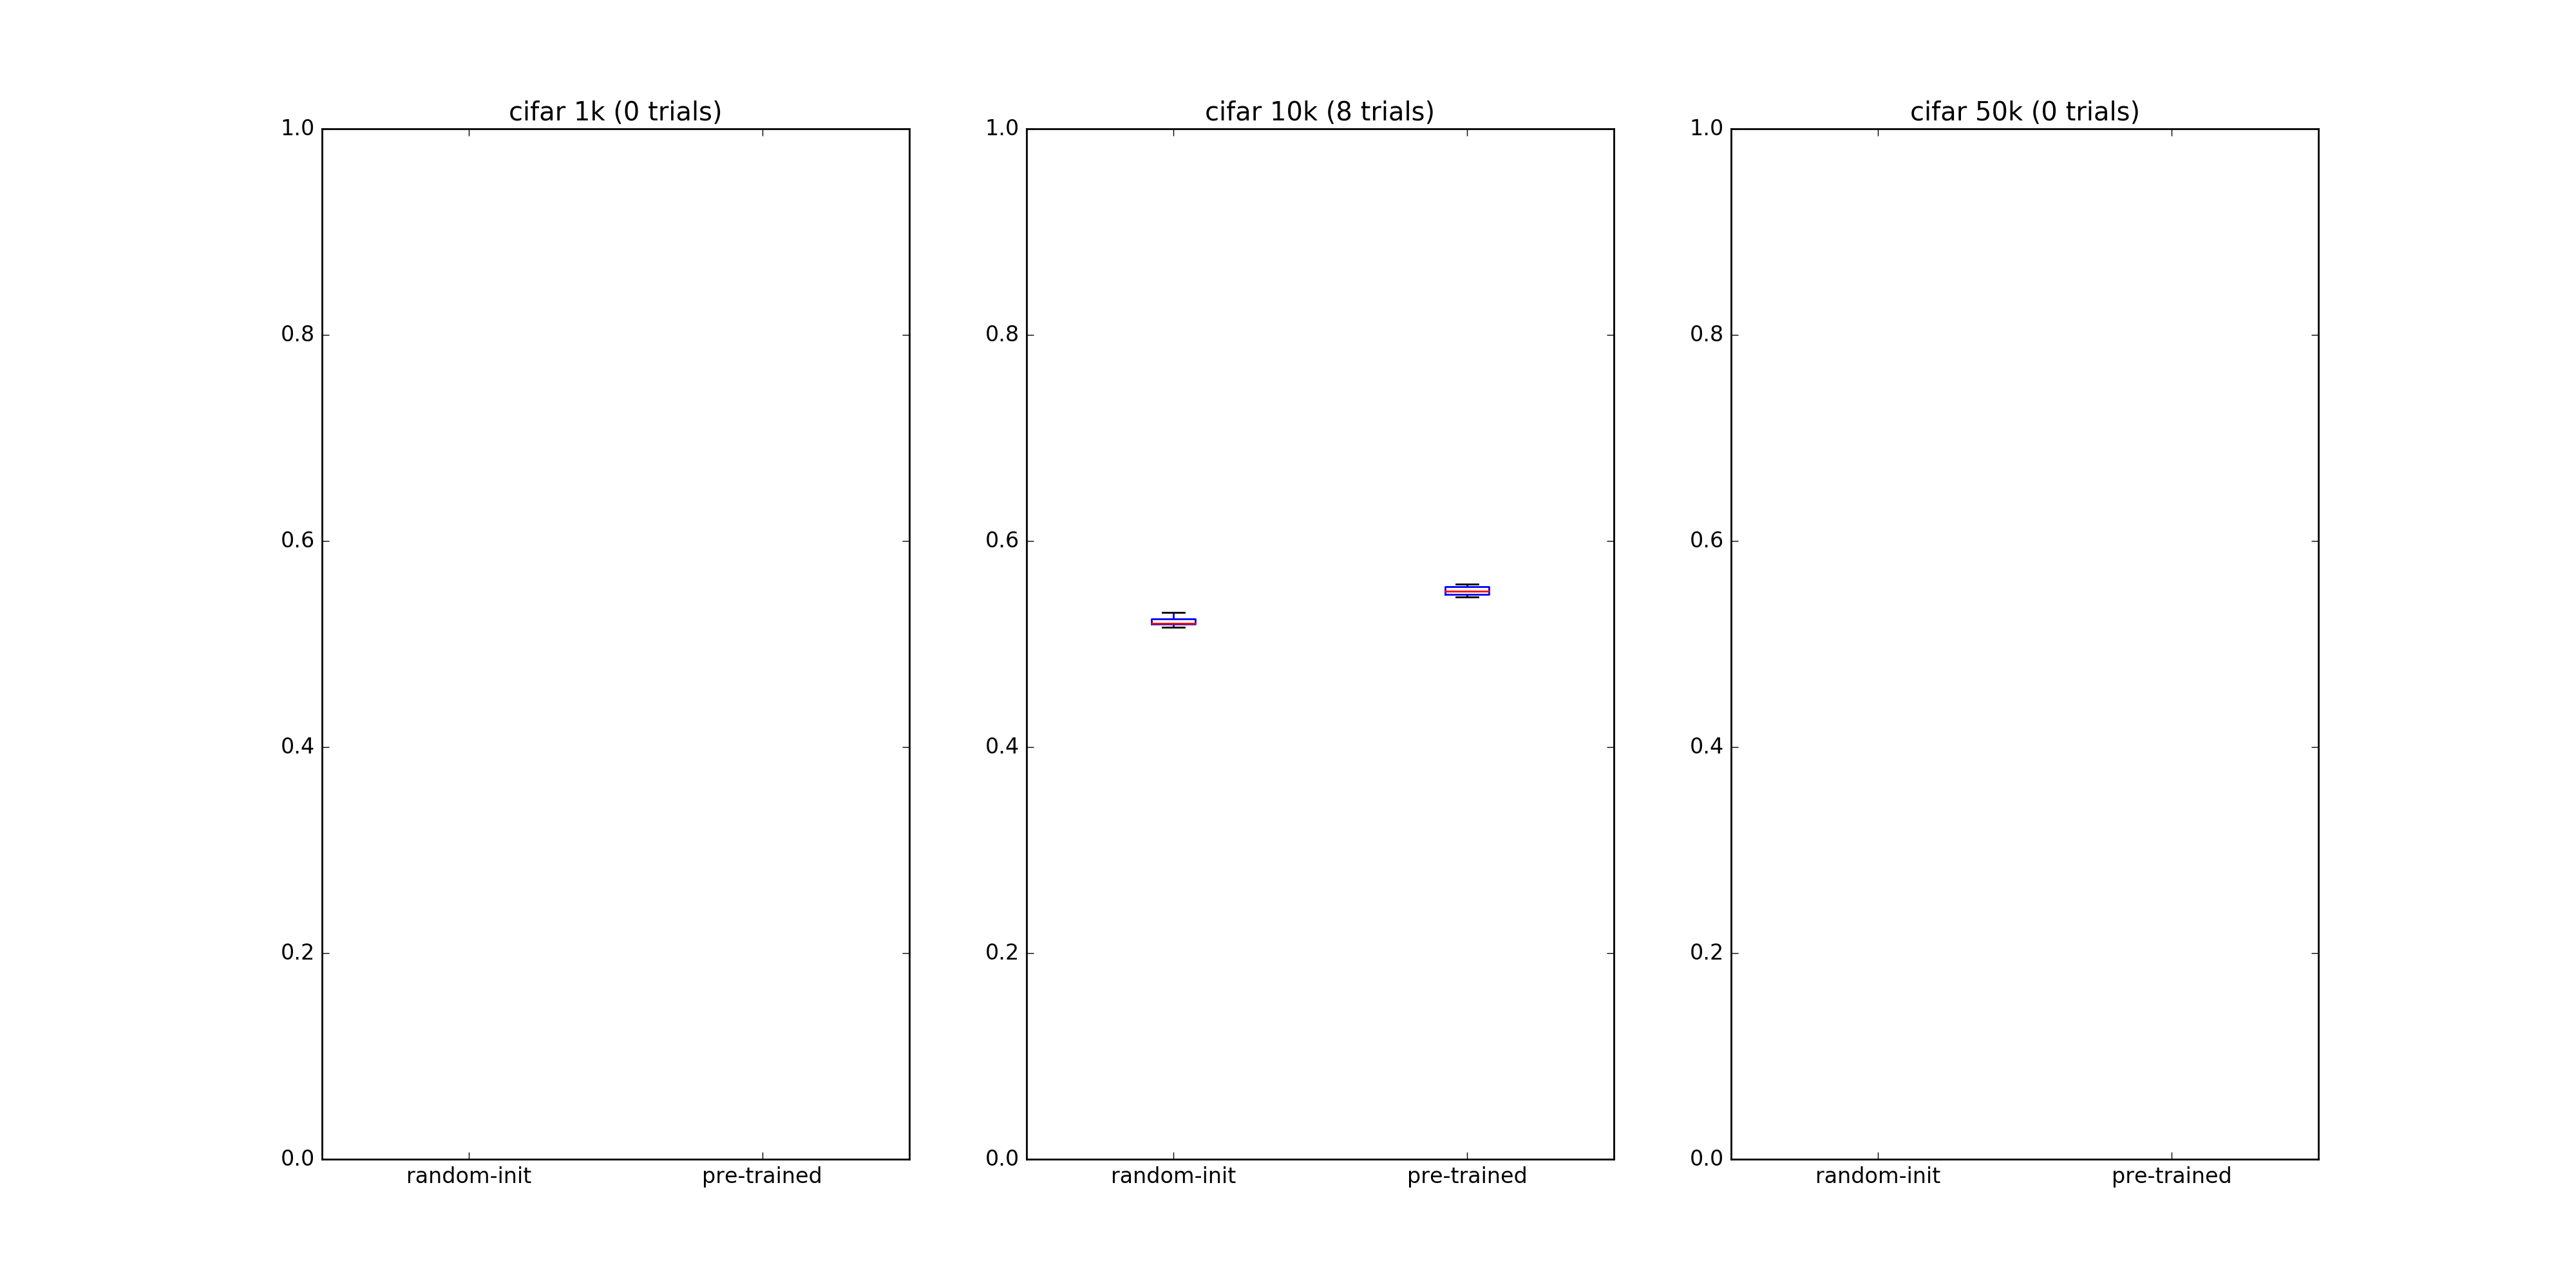
\includegraphics[width=\linewidth]{box_plots/boxplots_cifar.png}
\caption{boxplot of training accuracies}
\end{figure}

\end{block}

\end{column} % End of column 3

\begin{column}{\sepwid}\end{column} % Empty spacer column

\begin{column}{\onecolwid} % The third column

%----------------------------------------------------------------------------------------
%	CONCLUSION
%----------------------------------------------------------------------------------------

\begin{block}{CK+ Dataset}
\begin{figure}

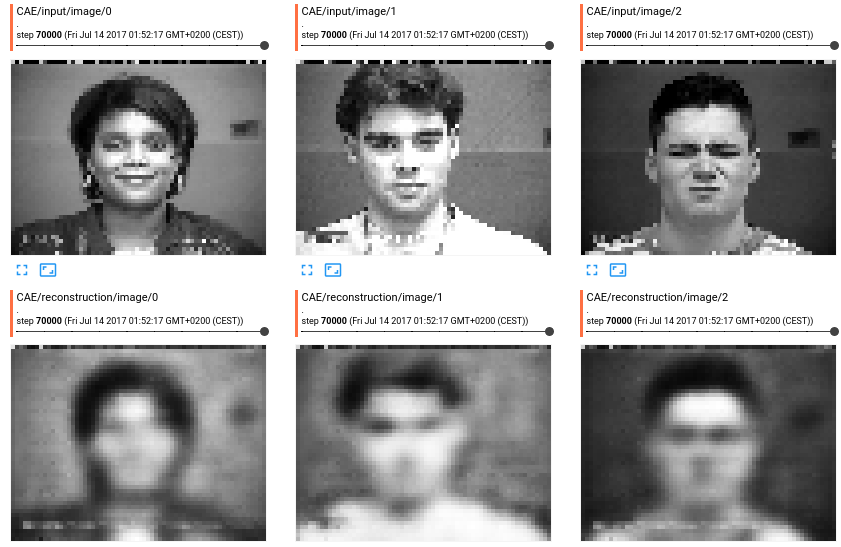
\includegraphics[width=0.8\linewidth]{graphics/ckplus_reconstructions_better.png}
\caption{Triángulos con ángulo común}
\end{figure}
Para que practiques te dejamos la siguiente lista de problemas relacionados con bisectrices.
%\begin{enumerate}

\end{block}

\begin{block}{Stats}
\begin{itemize}
\item (lmage content) facial expressions
\item (label type) emotions (TODO: nbr)
\item (datase sizes) extremely small set size (TODO: add numbers)
\item (size and colors) large (TODO: add size), 1 channel (grayscale) 
\item (compared difficulty) easier task but bigger images and very few images
\item (SOTA performance) include Sabbir
\item (extra: ) datapoints are sequences (explain our choice), cropping for smaller images

\end{itemize}
\end{block}

%\begin{block}{References}

%\nocite{*} % Insert publications even if they are not cited in the poster
%\small{\bibliographystyle{unsrt}
%\bibliography{sample}\vspace{0.75in}}

%\end{block}

%----------------------------------------------------------------------------------------

\end{column} % End of the third column

\end{columns} % End of all the columns in the poster

\end{frame} % End of the enclosing frame

\end{document}
